%--------------------------------------------------------------------
\medskip
\subsection{Realizar la implementación del proceso ETL para generar y poblar el modelo multidimensional diseñado en los apartados anteriores}
Para la realización de este apartado, se ha hecho uso de la herramienta Pentaho y se parte del JOB/Trabajo global \texttt{Global\_IMF\_def.kjb} proporcionado en el módulo de este caso práctico y que se encuentra situado en la carpeta \texttt{src/} y cuya estructura se muestra en la Figura \ref{Global_IMF}. En la carpeta \texttt{src/} se encuentran todos los ficheros fuente utilizados para el proceso ETL.

\begin{figure}[!th]
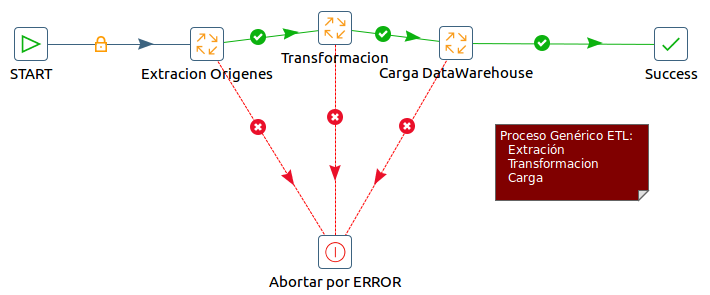
\includegraphics[scale=0.5]{Global_IMF.png}
\centering
\caption{Estructura del trabajo \texttt{Global\_IMF\_def}.}
\label{Global_IMF}
\end{figure}

A continuación se van a explicar en detalle cada uno de los trabajos en los que se divide este trabajo global:


%--------------------------------------------------------------------
\medskip
\subsubsection{Extracción Orígenes}
La estructura general de este trabajo se encuentra en el fichero \texttt{Global\_Extraccion.kjb} y se muestra en la Figura \ref{Global_Extraccion}.

\begin{figure}[!th]
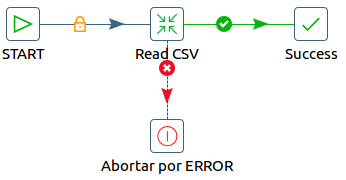
\includegraphics[scale=0.5]{Global_Extraccion.png}
\centering
\caption{Estructura del trabajo \texttt{Global\_Extraccion}.}
\label{Global_Extraccion}
\end{figure}

En este trabajo lo único que se hace es leer los datos que vienen proporcionados por la fuente de datos descrita en la sección \ref{01} y volcarlos todos en una tabla que servirá de entrada para el trabajo de Transformación explicado en la sección \ref{Transformacion}. Esto se hace a través de una transformación de Pentaho y que se encuentra en el fichero \texttt{Read\_CSV.ktr} y cuya estructura se muestra en la Figura \ref{Read_CSV}.

\begin{figure}[!th]
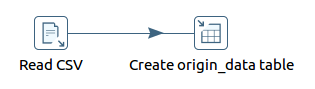
\includegraphics[scale=0.5]{Read_CSV.png}
\centering
\caption{Estructura de la transformación \texttt{Read\_CSV}.}
\label{Read_CSV}
\end{figure}


\newpage
%--------------------------------------------------------------------
\medskip
\subsubsection{Transformación}
\label{Transformacion}
La estructura general de este trabajo se encuentra en el fichero \texttt{Global\_Transformacion.kjb} y se muestra en la Figura \ref{Global_Transformacion}.

\begin{figure}[!th]
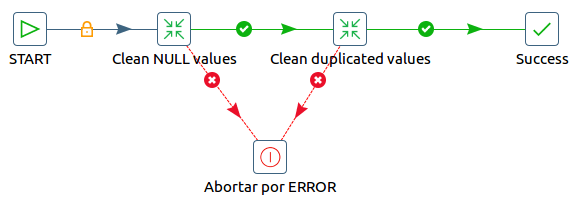
\includegraphics[scale=0.5]{Global_Transformacion.png}
\centering
\caption{Estructura del trabajo \texttt{Global\_Transformacion}.}
\label{Global_Transformacion}
\end{figure}

En este proceso se realizan dos transformaciones: una para eliminar aquellos registros con valores nulos y otra para eliminar aquellos registros que contengan claves primarias duplicadas. A continuación se explica cada una con mayor detalle:


%--------------------------------------------------------------------
\medskip
\subsubsection*{Eliminación valores nulos}
Como se definió en el modelo físico en la sección \ref{09}, en todas las tablas existe un campo como clave primaria (\texttt{PK}) y por definición, este campo no puede ser nulo. Por lo que se van a eliminar aquellos registros que contengan en alguno de los campos \texttt{PK} un valor \texttt{NULL}. Para ello, se hace uso de la transformación \texttt{Clean\_NULL\_values.ktr} y cuya estructura se muestra en la Figura \ref{NULL_values}.

\begin{figure}[!th]
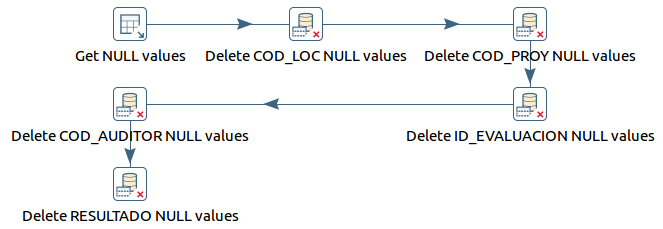
\includegraphics[scale=0.5]{Clean_NULL_values.png}
\centering
\caption{Estructura del trabajo \texttt{Clean\_NULL\_values}.}
\label{NULL_values}
\end{figure}

Además, para obtener estos registros, se hace uso de la siguiente sentencia SQL:
\lstinputlisting{code/SELECT_NULL_VALUES.sql}

Importante destacar que aunque el campo \texttt{RESULTADO} es una clave primaria, se trata del campo que se quiere analizar por el departamento antifraude, por lo que este tampoco puede ser nulo.


\newpage
%--------------------------------------------------------------------
\medskip
\subsubsection*{Eliminación claves primarias duplicadas}
Por definición, un valor de un campo que es clave primaria (\texttt{PK}) es único, ya que identifica de manera unívoca a cada registro. Pues siguiendo esta definición, se tiene que asegurar que en la fuente de datos no vienen registros distintos que hacen referencia a la misma clave primaria, lo cual duplicaría la clave primaria. Por ejemplo, supongamos que tenemos los siguientes registros, donde \texttt{codigo\_local} es la clave primaria:

\begin{center} 
\begin{table}[!th]
\begin{tabular}{|c|c|} \hline
\texttt{codigo\_local} & \texttt{nombre\_local} \\ \hline
1 & Pepito \\ \hline
1 & Menganito \\ \hline 
\end{tabular}
\centering
\end{table}
\end{center}

En este caso, si se intentan insertar ambos registros en la tabla \texttt{CLIENTE}, saltará un error diciendo que el valor \texttt{1} está duplicado. Como no podemos quedarnos con uno, porque no sabemos cuál es el correcto y cuál el erróneo, tenemos que eliminar ambos.\\

Siguiendo esta filosofía, se hace la transformación \texttt{Clean\_duplicated\_values.ktr} y cuya estructura se muestra en la Figura \ref{duplicated_values}.

\begin{figure}[!th]
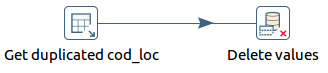
\includegraphics[scale=0.5]{Clean_duplicated_values.png}
\centering
\caption{Estructura del trabajo \texttt{Clean\_duplicated\_values}.}
\label{duplicated_values}
\end{figure}

Además, para obtener estos registros, se hace uso de la siguiente sentencia SQL:
\lstinputlisting{code/SELECT_DUPLICATED_VALUES.sql}




%--------------------------------------------------------------------
\medskip
\subsubsection{Carga DataWarehouse}
Por último, tras realizar las transformaciones hay que realizar la carga del DataWarehouse. Para ello, se hace uso del trabajo \texttt{Global\_Carga.kjb} y cuyo esquema se muestra en la Figura \ref{Global_Carga}.

\begin{figure}[!th]
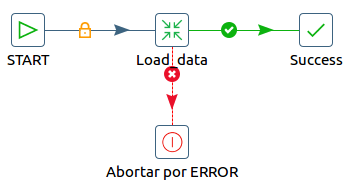
\includegraphics[scale=0.5]{Global_Carga.png}
\centering
\caption{Estructura del trabajo \texttt{Global\_Carga}.}
\label{Global_Carga}
\end{figure}

\newpage
Este trabajo lo que hace es crear cada una de las tablas definidas en la sección \ref{09} con los datos que ya han sido transformados. Para ello, hace uso de la transformación \texttt{Load\_data} cuyo estructura se muestra en la Figura \ref{Load_data}


\begin{figure}[!th]
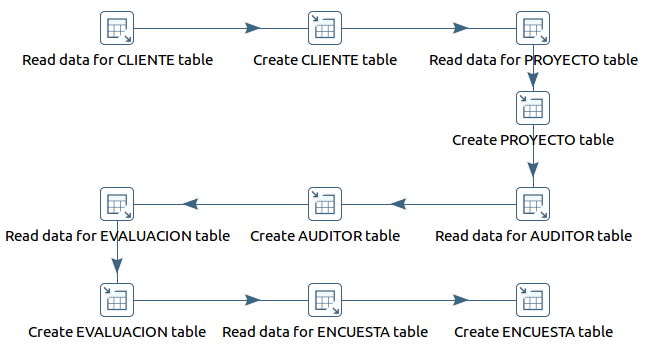
\includegraphics[scale=0.5]{Load_data.png}
\centering
\caption{Estructura de la transformación \texttt{Load\_data}.}
\label{Load_data}
\end{figure}

Las sentencias SQL necesarias para crear cada una de las tablas se muestran a continuación:
\lstinputlisting{code/CREATE_TABLES.sql}

Es importante destacar aquí que en la creación de la tabla \texttt{ENCUESTA} no se definen los campos \texttt{CLIENTE}, \texttt{PROYECTO}, \texttt{AUDITOR} y \texttt{EVALUACION} como claves foráneas (\texttt{FK}) porque al intentar lanzar el proceso entero y borrar todas las tablas con un \texttt{TRUNCATE} como hace Pentaho, da error por las restricciones de clave foránea, incluso si se pone \texttt{ON DELETE SET NULL} en la definición sigue dando el mismo error. Sin embargo, al rellenar la tabla, se hace uso de las claves primarias definidas.
